\documentclass[a4paper]{article}
\usepackage[utf8]{inputenc}
\usepackage[T1]{fontenc}
\usepackage{graphics}
\usepackage{libertine}
\usepackage[french]{babel}
\usepackage{tabularx}
\usepackage{geometry}
\usepackage{xcolor}
\usepackage{mathtools}

\newlength\cardheight
\newlength\cardwidth
\setlength\cardheight{87mm}
\setlength\cardwidth{56mm}

\newlength\cardhspace
\newlength\cardvspace
\setlength\cardhspace{56.5mm}

\def\tabularxcolumn#1{m{#1}}

\newcommand{\card}[3]{%
  %\textcolor{lightgray}{\rule{\cardwidth}{\cardheight}}%
  \begin{minipage}[t][\cardheight][t]{\cardwidth}%
    \begin{center}
      \vspace{03mm}
      {\textbf{\large \textsc{#1}}} \\
      \vspace{10mm}
      \begin{tabularx}{0.90\linewidth}{ m{1cm} X }
        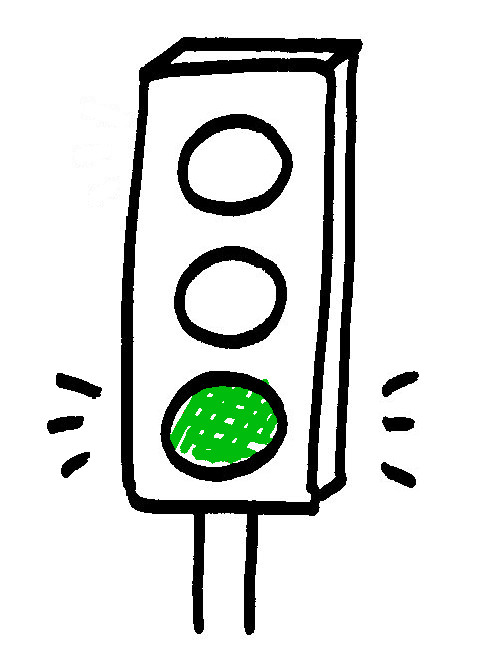
\includegraphics[width=10mm]{includes/feu-vert.jpg} & #2 \\
        \\
        
\includegraphics[width=10mm]{includes/feu-rouge.jpg} & #3 \\
      \end{tabularx}
    \end{center}
  \end{minipage}%
}

\newcommand{\cropmarktop}{
  \noindent%
  \rule{8mm}{1pt}%
  \hspace{2mm}%
  \clap{\rule[2mm]{1pt}{8mm}}%
  \hspace{\cardhspace}%
  \clap{\rule[2mm]{1pt}{8mm}}%
  \hspace{\cardhspace}%
  \clap{\rule[2mm]{1pt}{8mm}}%
  \hspace{\cardhspace}%
  \clap{\rule[2mm]{1pt}{8mm}}%
  \hspace{2mm}%
  \rule{8mm}{1pt}\\%
  \hspace*{1cm}%
}

\newcommand{\cropmarkmiddle}{
  \\[-1em]
  \rule{8mm}{1pt} \hfill \rule{8mm}{1pt}\\%
  \hspace*{1cm}%
}

\newcommand{\cropmarkbottom}{
  \\[-1em]
  \rule[-0.5pt]{8mm}{1pt} \hfill \rule[-0.5pt]{8mm}{1pt}\\[1mm]
  \hspace*{1cm}%
  \clap{\rule{1pt}{8mm}}%
  \hspace{\cardhspace}%
  \clap{\rule{1pt}{8mm}}%
  \hspace{\cardhspace}%
  \clap{\rule{1pt}{8mm}}%
  \hspace{\cardhspace}%
  \clap{\rule{1pt}{8mm}}%
}


\begin{document}


lien : https://labs.spotify.com/2014/09/16/squad-health-check-model/


\section{Squad Health Check model}

basé sur la version 1, September 2014
Traduction :
\begin{itemize}
\item Séverin Legras
\item Hervé Taboucou
\item Thomas Clavier
\end{itemize}

\subsection{De quoi s'agit-il?}

\begin{itemize}
\item Un atelier et une technique de visualisation aidant les équipes (squads) à s'améliorer.
\end{itemize}

\subsection{Audience}

\begin{itemize}
\item L'équipe elle-même
\item Les personnes apportant leur support à l'équipe (managers, coachs, etc.)
\end{itemize}

\subsection{Comment utiliser ce modèle}

\begin{itemize}
\item Imprimez et plastifiez les cartes.


\begin{itemize}
\item Page 2-5 = Cartes de questions (double face)
\item Page 6-9 = Cartes de vote (double face)
\end{itemize}
\item Rassemblez tous les membres de l'équipe dans la même salle
\item Discutez sur les cartes de questions. Chacune d'entre elle est un indicateur de bonne santé, accompagné d'un exemple de très bonne performance et d'un exemple particulièrement inefficace.
\item Demander à l'équipe comment elle se positionne sur chacun de ces indicateurs, en utilisant une méthode favorisant les décisions de groupe (par exemple: avec les cartes de vote).


\begin{itemize}
\item Un ``Feu Vert'' ne signifie pas un état parfaitement idéal, mais que l'équipe est satisfaite sur cet indicateur et ne voit pas d'amélioration significative à mettre en oeuvre dans l'immédiat.
\item Un ``Feu Orange'' signifie qu'il y a des problèmes importants qui nécessitent l'attention, mais ils ne constituent pas une situation irrécupérable.
\item Un ``Feu Rouge'' signifie que la situation est critique, et nécessite une amélioration immédiate.
\end{itemize}
\item Discutez les tendances d'évolution de ces indicateurs (la situation s'améliore-t-elle? Est-elle stable ou se dégrade-t-elle?)
\item Matéralisez visuellement les résultats de ces discussions.
\item Utilisez des données quantitatives (estimation, mesures, extrapolation\ldots{}) pour aider l'équipe à s'améliorer.
\item \subsection{Idées de mises en oeuvre}
\item Les cartes sont uniquement un point de départ pour initialiser des conversations productives. L'équipe doit se sentire libre d'ajouter/ôtre/modifier toute question afin de correspondre à ce qu'elle considère comme important pour elle.
\item Il est essentiel de s'assurer que cet outil soit utilisé en support de l'équipe dans son amélioration et surtout pas pour l'évaluer.
\end{itemize}

Le terme ``squad''  (retraduit ici par ``équipe'') est le mot utilisé par Spotify pour une équipe de développement petite, cross-fonctionnelle et auto-organisée.


\section{Cartes de questions}
\newgeometry{margin=10mm}
\thispagestyle{empty}

\cropmarktop%
%
\card{Livraison de valeur}
  {Nous livrons des produits extraordinaires! Nous en sommes fiers et nos clients en sont particulièrement contents.}
  {Ce que nous livrons est nul. Nous en avons honte. Nos clients nous détestent.}
%
\card{facilité de livraison}
  {Le processus de livraison est simple, sûr, indolore et quasiement totalement automatisé.}
  {Le processus de livraison est risqué, douloureux, nécessite beaucoup d'interventions manuelles, qui prennent énorméménet de temps.}
%
\card{Fun}
  {Nous aimons aller travailler le matin, et avons beaucoup de fun à travailler ensemble.}
  {Ennui\ldots{}.}
%
\cropmarkmiddle%
%
\card{Bonne santé du code}
  {Nous sommes fiers de la qualité de notre code. Il est propre, facile à lire et a une grande couverture de tests.}
  {Notre code est un tas de fumier et notre dette technique croît de façon incontrôlable.}
\card{Apprentissage}
  {Nous apprenons à chaque instant quelque chose d'intéressant.}
  {Nous n'avons jamais le temps d'apprendre quoi que ce soit.}
\card{Mission}
  {Nous savons exactement pourquoi nons sommes là, et nous sommes passionnés en connaissance de cause.}
  {Nous ne savons pas pouquoi nous sommes là, il n'y a pas de schéma général  ou d'orientation globale. Nos ``missions'' sont totalement floues et démotivantes.}
%
\cropmarkbottom

\clearpage
\cropmarktop%
%
\card{Acteurs\ldots{} ou pions\ldots{}}
 {Nous contrôlons notre destin. Nous décidons ce que nous développons et comment nous le développons.}
 {Nous ne sommes que des pions sur un échiquier, et nous n'avons aucune influence sur ce que nous construisons et comment nous le développons.}
\card{Vélocité}
  {Nous faisons immédiatement ce que nous avons décidé. Pas d'attente, pas de délai.}
  {Nous ne finissons jamais rien. Nous sommes systématiquement bloqués et interrompus. En particuliern les user stories sont bloqués par les dépendances critiques d'autres produits.}
\card{Processus adapté}
  {Notre façon de travailler nous correspond tout à fait !}
  {Notre façon de travailler est ridicule.}
%
\cropmarkmiddle%
%
\card{Support}
  {Nous obtenons toujours du support et de l'aide de nos sponsors dès que nous le demandons.}
  {Nous sommes régulièrement bloqués car nous ne pouvons obtenir du soutien et de l'aide de la part de nos sponsor quand nous le demandons.}
%
\card{Travail d'équipe}
  {Nous sommes un groupe qui a vraiment pris une forme d'équipe, avec un niveau de collaboration extraodinaire.}
  {Nous sommes une bande d'individus qui ne se connaissent pas et nous ne sous soucions pas de savoir ce que les autres font.}
%
\cropmarkbottom



\restoregeometry


\end{document}
